\documentclass[a4paper,12pt]{article}

\title{

    \begin{figure}[H]
    \centering
    
\includegraphics{../../mak_logo.png}
    \end{figure}
    \textbf {COLLEGE OF ENGINEERING, DESIGN, ART AND TECHNOLOGY\\
    DEPARTMENT OF ELECTRICAL AND COMPUTER ENGINEERING\\
    SCHOOL OF ENGINEERING}\\

}

\usepackage{listings}
\usepackage{fancyhdr}
\usepackage[utf8]{inputenc}
\usepackage{hhline}
\usepackage{float}
\usepackage{graphicx}
\usepackage{lastpage}
\usepackage[top=2cm,bottom=2cm,left=2cm,right=2cm]{geometry}

% include footers
\pagestyle{fancy}
\lfoot{Shawal Mbalire} 
\rfoot{21/U/0851}
\cfoot{Page~\thepage~of \pageref{LastPage}}


\begin{document}
\maketitle

\vfil
\begin{center}
BACHELOR OF SCIENCE IN ELECTRICAL ENGINEERING\\[20pt]
ELE2111 MATLAB ASSIGNMENT\\[20pt]

SHAWAL MBALIRE\\
21/U/0851 \\
\end{center}
\newpage




\subsubsection*{Question 1\\
Plot the Bode magnitude and phase for the system with transfer function \[ G_{(s)} = \frac{2000(s + 0.5)} {s(s + 10)(s + 50)}\]}

First we expand the function as a polynomial as matlab uses the polynomial version of the transfer function. 
\[ G_{(s)} = \frac{2000\times s + 2000\times0.5} {s(s\times s + 10\times s + 50\times s + 10\times50)}\]
\[ G_{(s)} = \frac{2000s + 1000} {s(s^2 + 10s + 50s + 500)}\]
\[ G_{(s)} = \frac{2000s + 1000} {s^3 + 60s^2 + 500s}\]
The polynomial is then used to create a transfer function. The transfer function is then plotted using the bode function. The code is shown below.

\begin{lstlisting}[language=Matlab]

    % Define the transfer function
    numerator = [2000, 1000];
    denominator = [1, 60, 500, 0];
    
    % Create a transfer function
    sys = tf(numerator, denominator);
    
    % Plot the Bode plot
    figure;
    bode(sys);
    title('Bode Plot');
    grid on;
  

\end{lstlisting}

The resulting figure is shown below

\begin{figure}[H]
    \centering
    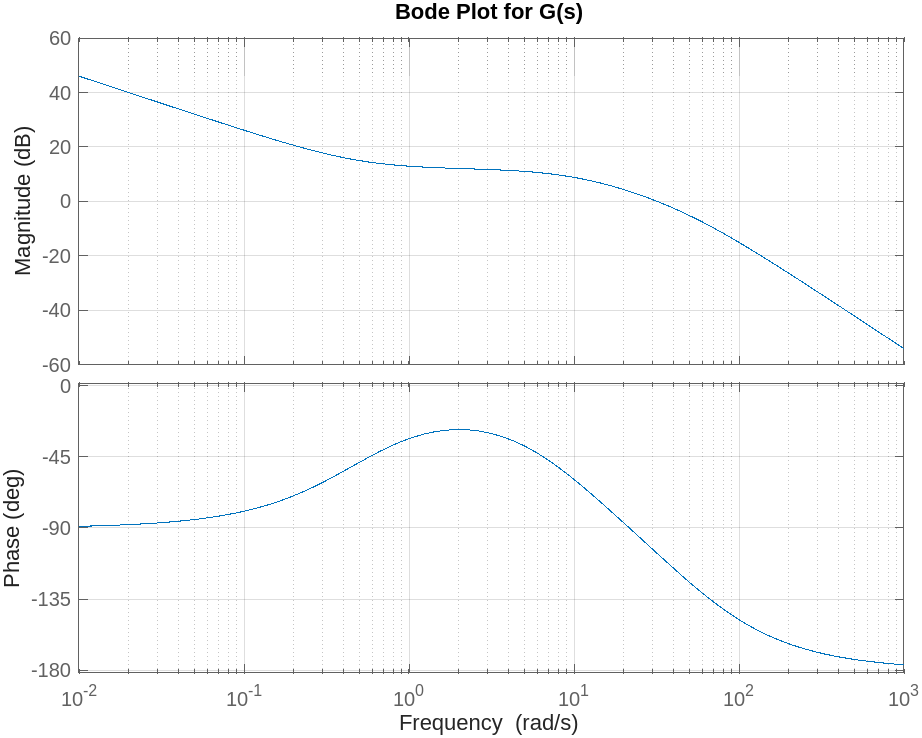
\includegraphics[width=\linewidth]{q1.png}
    \caption{Bode plot for G (s)}\label{fig:q1}
\end{figure}





\subsubsection*{Question 2\\Sketch the Bode plot (Magnitude and Phase Angle) for \[ H = \frac{10000(S + 1)} {(S + 10)(S + 1000)}\]} 

First we expand the function as a polynomial as matlab uses the polynomial version of the transfer function.
\[ H = \frac{10000(S + 1)} {(S + 10)(S + 1000)}\]
\[ H = \frac{10000S + 10000} {S^2 + 1010S + 10000}\]
The polynomial is then used to create a transfer function. The transfer function is then plotted using the bode function. The code is shown below.

\begin{lstlisting}[language=Matlab]
    % Define the transfer function
    numerator_H = [10000, 10000];  % 10000(S + 1)
    denominator_H = [1, 1010, 10000];  % (S + 10)(S + 1000)

    % Create a transfer function
    sys_H = tf(numerator_H, denominator_H);

    % Plot the Bode plot
    figure;

    % Bode magnitude plot
    bode(sys_H);
    title('Bode Magnitude Plot for H(s)');
    grid on;

\end{lstlisting}

The resulting figure is shown below

\begin{figure}[H]
    \centering
    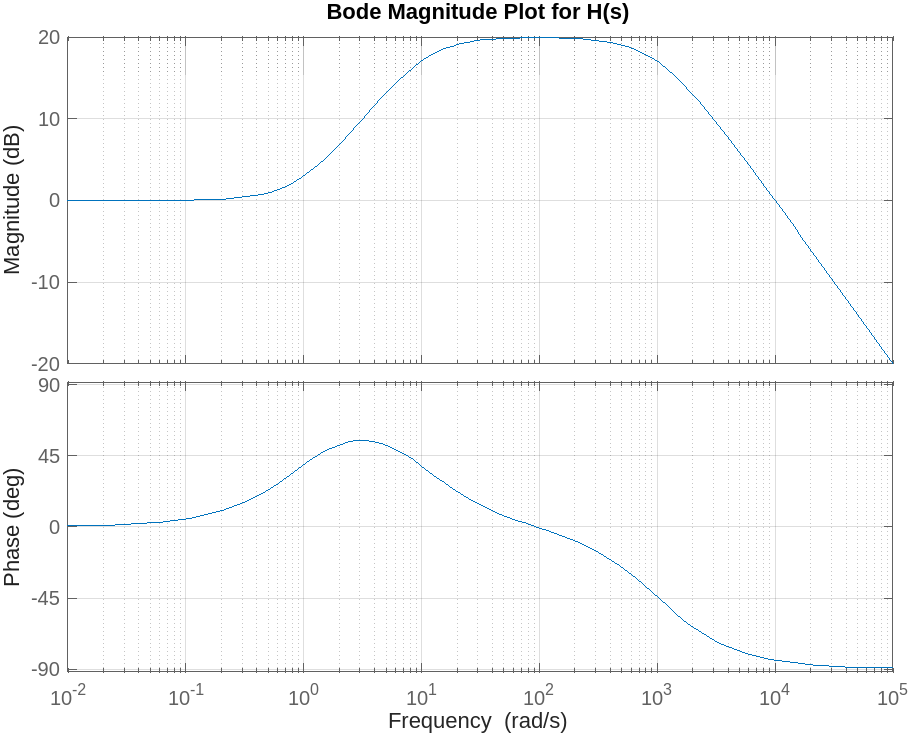
\includegraphics[width=\linewidth]{q2.png}
    \caption{Bode plot for a H (s)}\label{fig:q2}
\end{figure}






\subsubsection*{Question 3\\Plot a Bode plot of a highpass filter with a gain of 0 dB and cutoff frequency of 3000 Hz.}

Assume a first order continous implementation of a high pass filter. The transfer function is given by 
\[ H = \frac{s\tau}{s\tau +1}\]
\[ f = \frac{1}{2\pi\tau}\]
\[ \tau = \frac{1}{2\pi f} \]
\[ H = \frac{s\frac{1}{2\pi f}}{s\frac{1}{2\pi f} +1}\]
\[ H = \frac{s}{s + 2\pi f}\]

\[ H = \frac{s}{s + 6000\pi}\]

\[DC~Gain = \lim_{s\rightarrow 0} s\times \frac{s}{s + 6000\pi}\]
\[DC~Gain = 0\]

The code is shown below.
\begin{lstlisting}

    gain = 0;  % Gain in dB
    cutoff_frequency = 3000;  % Cutoff frequency in Hz

    % Create a highpass filter transfer function
    numerator_highpass = [1, 0];  % (s)
    denominator_highpass = [1, 2 * pi * cutoff_frequency];  % (s + 2*pi*f)

    % Create a transfer function
    sys_highpass = tf(numerator_highpass, denominator_highpass);

    % Plot the Bode plot
    figure;

    % Bode magnitude plot
    bode(sys_highpass);
    title('Bode Plot for Highpass Filter');
grid on;

\end{lstlisting}

The resulting figure is shown below

\begin{figure}[H]
    \centering
    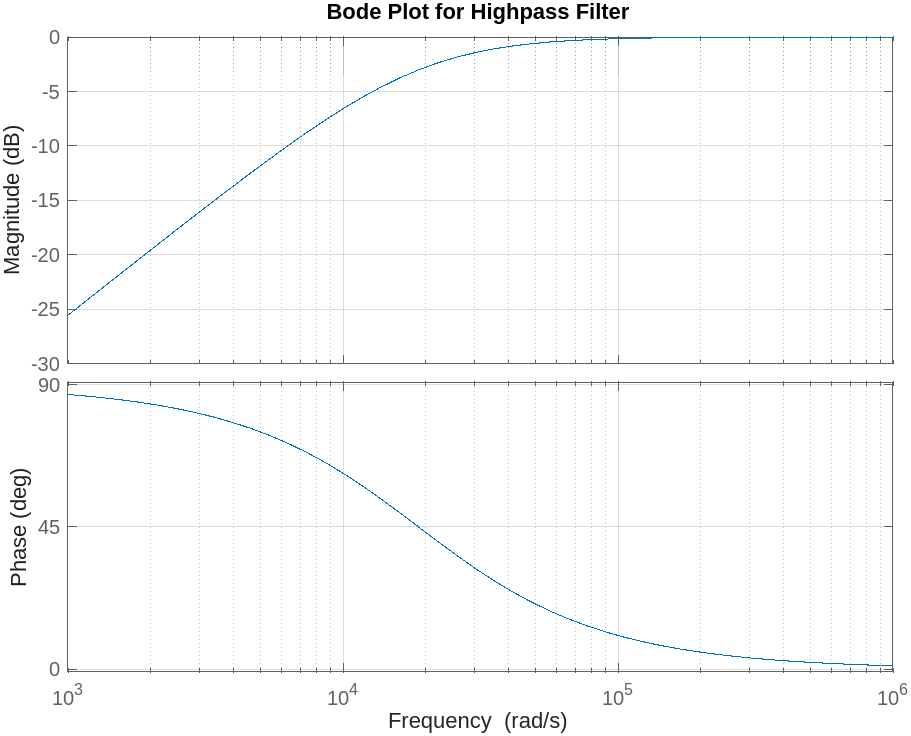
\includegraphics[width=\linewidth]{q3.png}
    \caption{Bode plot for a highpass filter}\label{fig:q3}
\end{figure}

\end{document}